\chapter{Gestion de la température}

Pour réaliser les différentes expériences prévues, il est essentiel de pouvoir contrôler la température du capteur QCM.  
La plage de température souhaitée est de 15 à 50°C, sachant que la température maximale supportée par le capteur est de 75°C \cite{manual-openqcmQ1}.

\section{Choix de la méthode de refroidissement}

Plusieurs méthodes ont été envisagées :
\begin{itemize}[label=\textbullet]
    \item Placer le capteur dans un réfrigérateur ou un congélateur.
    \item Utiliser des modules Peltier pour créer un système de refroidissement.
    \item Faire circuler un fluide plus froid ou plus chaud que la température ambiante autour du module électrochimique via un tuyau.
\end{itemize}

La première méthode a été écartée car elle ne permet pas de contrôler précisément la température, et il existait un risque d’endommager le capteur en le refroidissant en dessous de 0°C. De plus, cette solution ne permet pas de chauffer le capteur au-delà de la température ambiante.

La seconde méthode, utilisant des modules Peltier, a été écartée en raison de la complexité de mise en œuvre, du temps limité pour ce travail, ainsi que du coût des composants.

La troisième méthode a été retenue car elle est simple à mettre en œuvre, d’autant plus qu’une pompe de circulation était déjà disponible. De plus, la pompe péristaltique utilisée permet de régler le débit du fluide circulant, ce qui autorise un contrôle de la vitesse de refroidissement, et donc de la température du capteur.

\section{Schéma de montage}

Avant de pouvoir réaliser des mesures sur la gélatine, il est essentiel de refroidir le liquide à une température inférieure à 20°C pour initier la gélification.  
Pour cela, un bain de glace est utilisé. Le liquide est placé dans le récipient en verre du module électrochimique.  
Grâce à un tuyau en silicone et à une pompe péristaltique, le liquide circule autour du récipient.  
Le tuyau est enroulé autour du récipient, formant ainsi un échangeur de chaleur.  
Ce tuyau flexible en silicone, d’un diamètre extérieur de 4 mm, effectue quatre tours autour du récipient.  
Le tuyau est maintenu en place par un clip imprimé en 3D.

\begin{figure}[H]
    \centering
    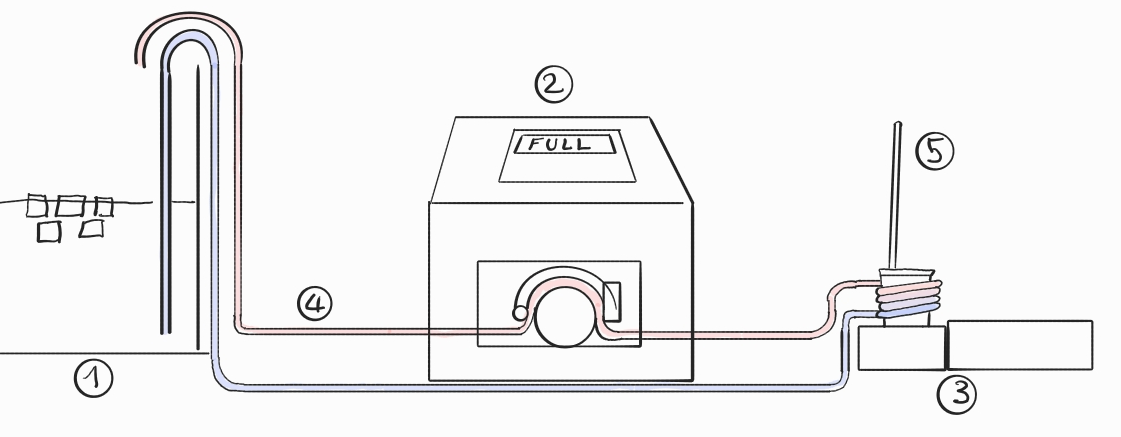
\includegraphics[width=\textwidth]{assets/figures/Pump TB.png}
    \caption{Schéma de refroidissement du module QCM}
    \label{fig:Shema_glacière}
\end{figure}

\begin{enumerate}
    \item Bain de glace ou bain chauffant
    \item Pompe péristaltique
    \item Récipient en verre du module QCM
    \item Tuyau flexible en silicone
    \item Thermomètre ou sonde de température PT100
\end{enumerate}

Pour chauffer le mélange lorsque la température doit être supérieure à la température ambiante, le bain de glace est remplacé par un bain chauffant réglable.

\section{Maintien du tuyau}

Pour maintenir le tuyau en place, un clip a été conçu et imprimé en 3D.  
Le clip est composé de quatre sections circulaires qui permettent de glisser le tuyau flexible à l’intérieur tout en empêchant sa sortie accidentelle.  
Les clips ont été imprimés en ABS afin de résister à la chaleur.

\begin{figure}[H]
    \centering
    \includegraphics[width=\textwidth]{assets/figures/ATACHE TUBE V2.png}
    \caption{Clip de maintien du tuyau autour du récipient}
    \label{fig:Clip_tuyau}
\end{figure}

\section{Isolation thermique}

Un isolant thermique composé de papier bulle et de scotch est utilisé pour envelopper le récipient en verre, afin de réduire au maximum les pertes thermiques par convection entre le récipient et l’air ambiant.

\begin{figure}[H]
    \centering
    \begin{minipage}{0.48\textwidth}
        \centering
        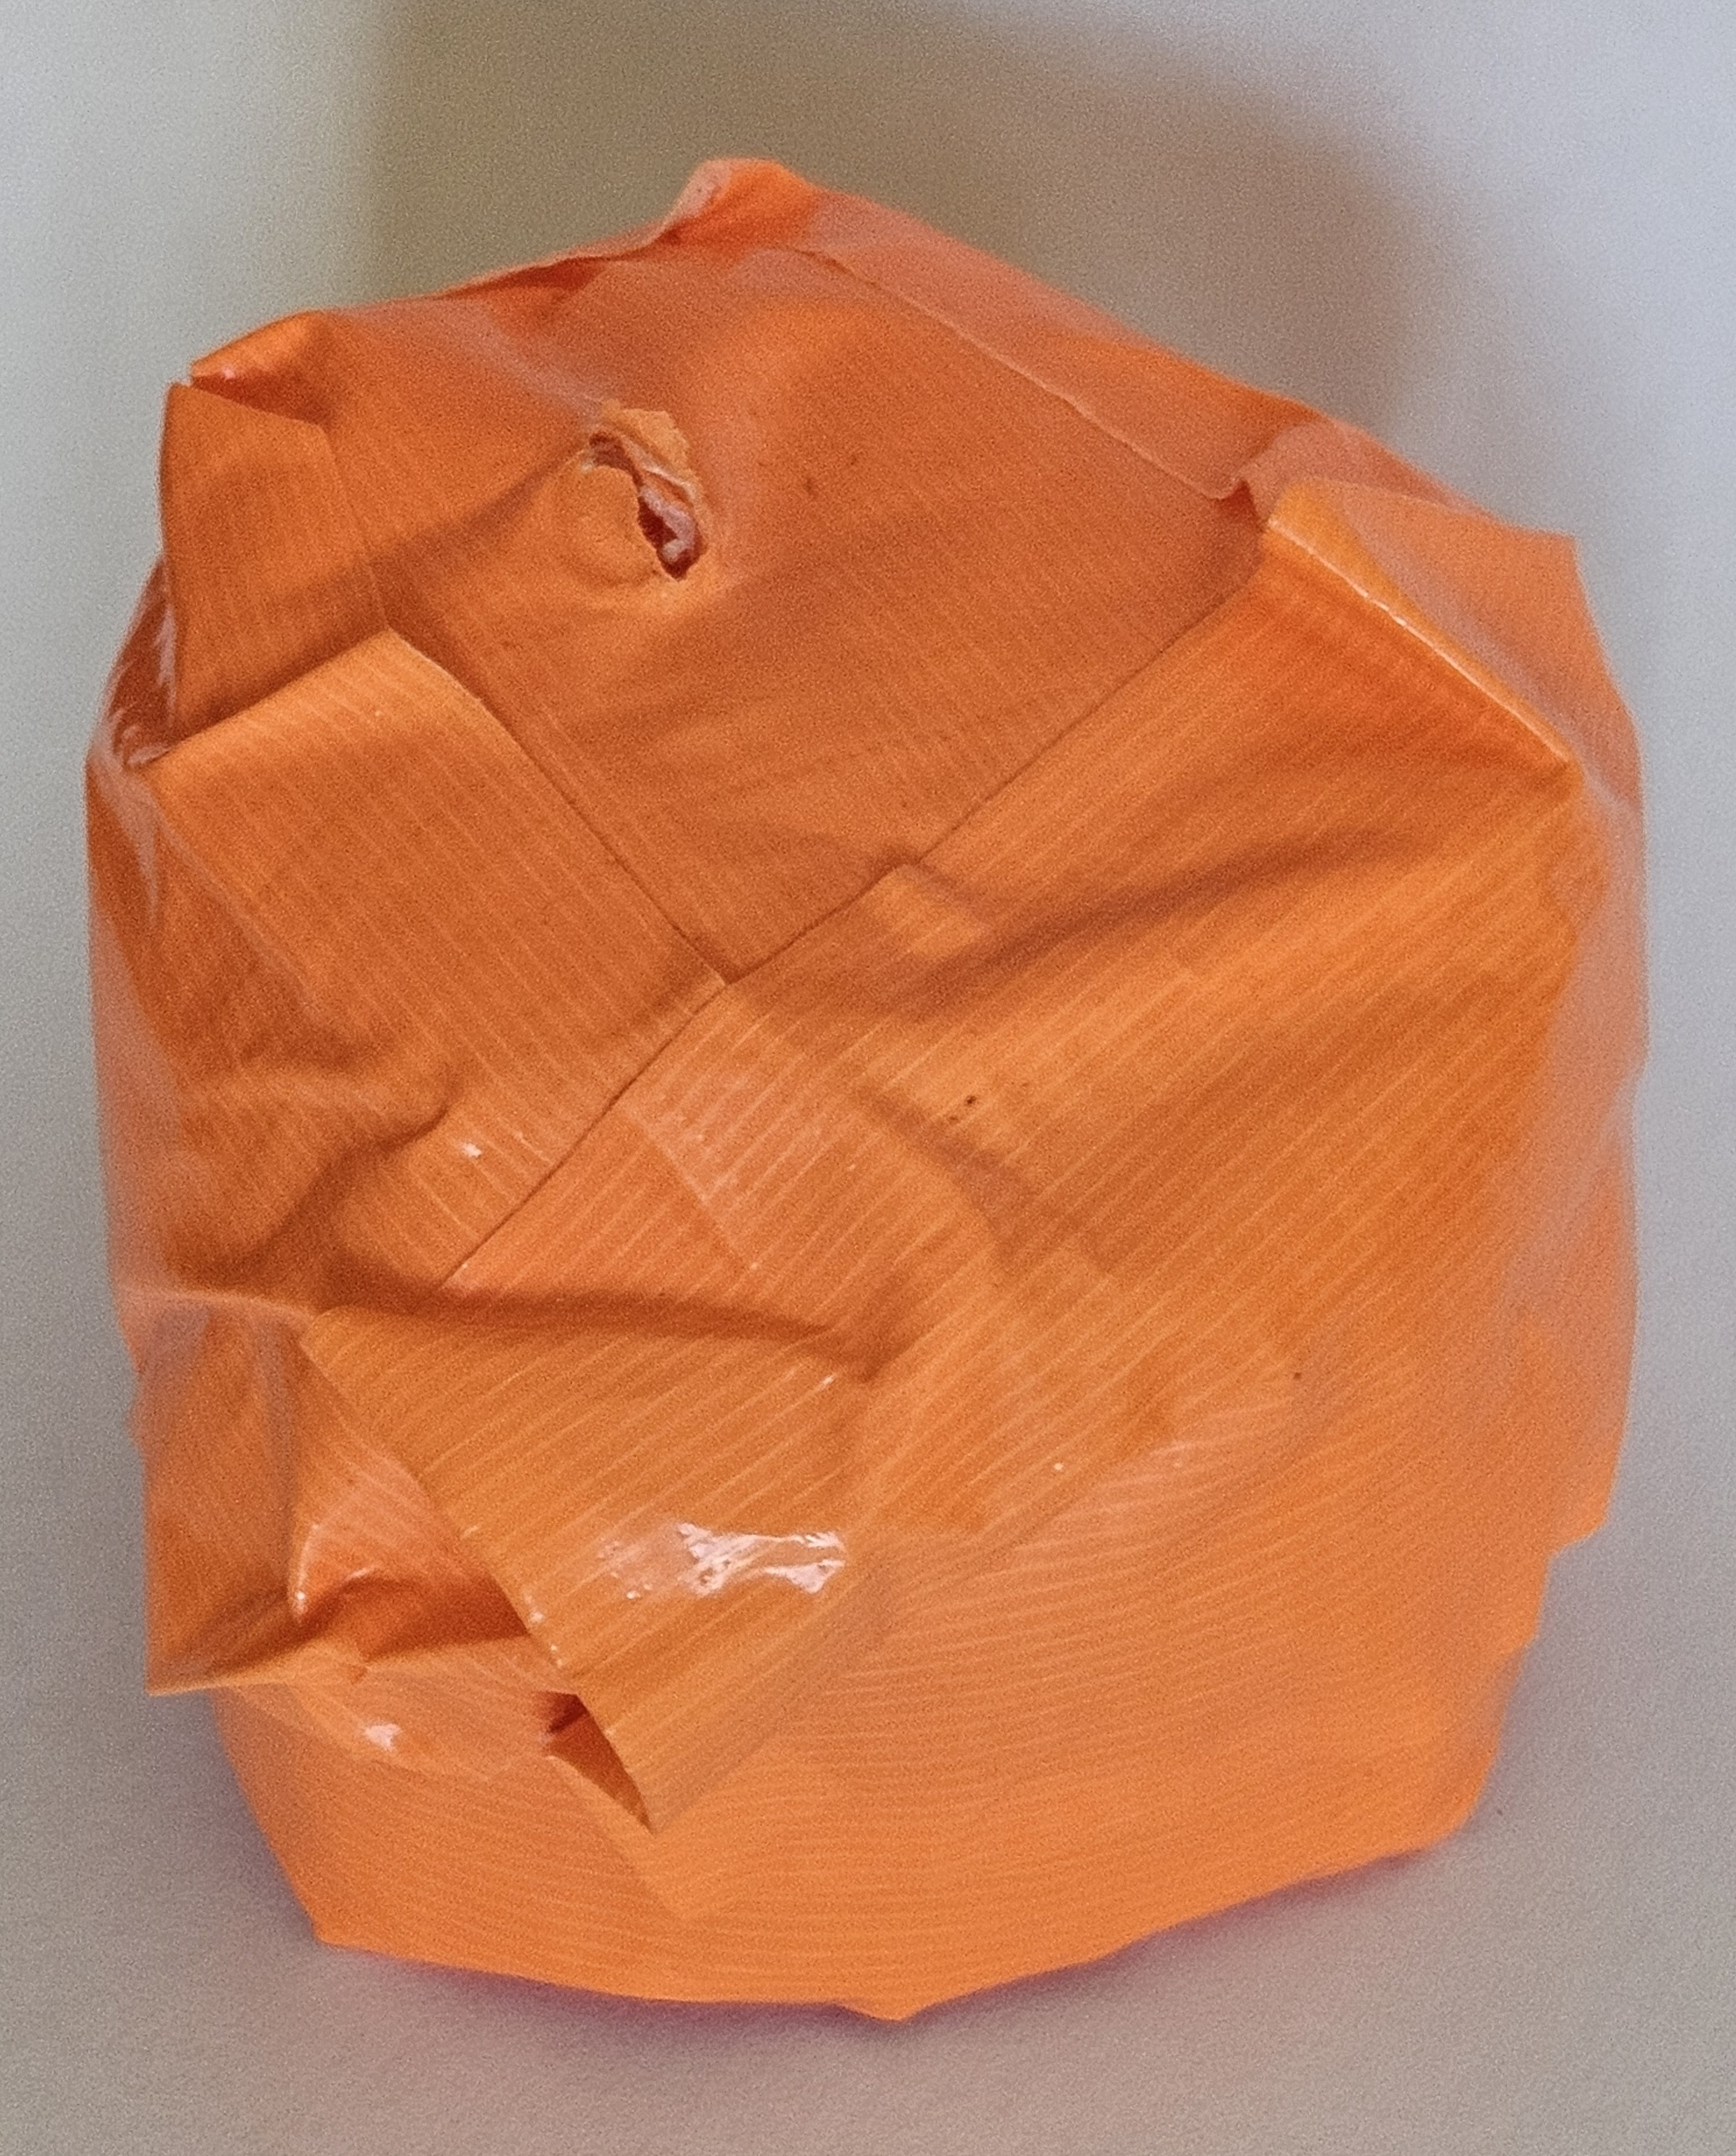
\includegraphics[width=\textwidth]{assets/figures/Exterieur_Isolant.jpg}
        \caption{Extérieur de l'isolant thermique}
        \label{fig:Exterieur_Isolant}
    \end{minipage}\hfill
    \begin{minipage}{0.48\textwidth}
        \centering
        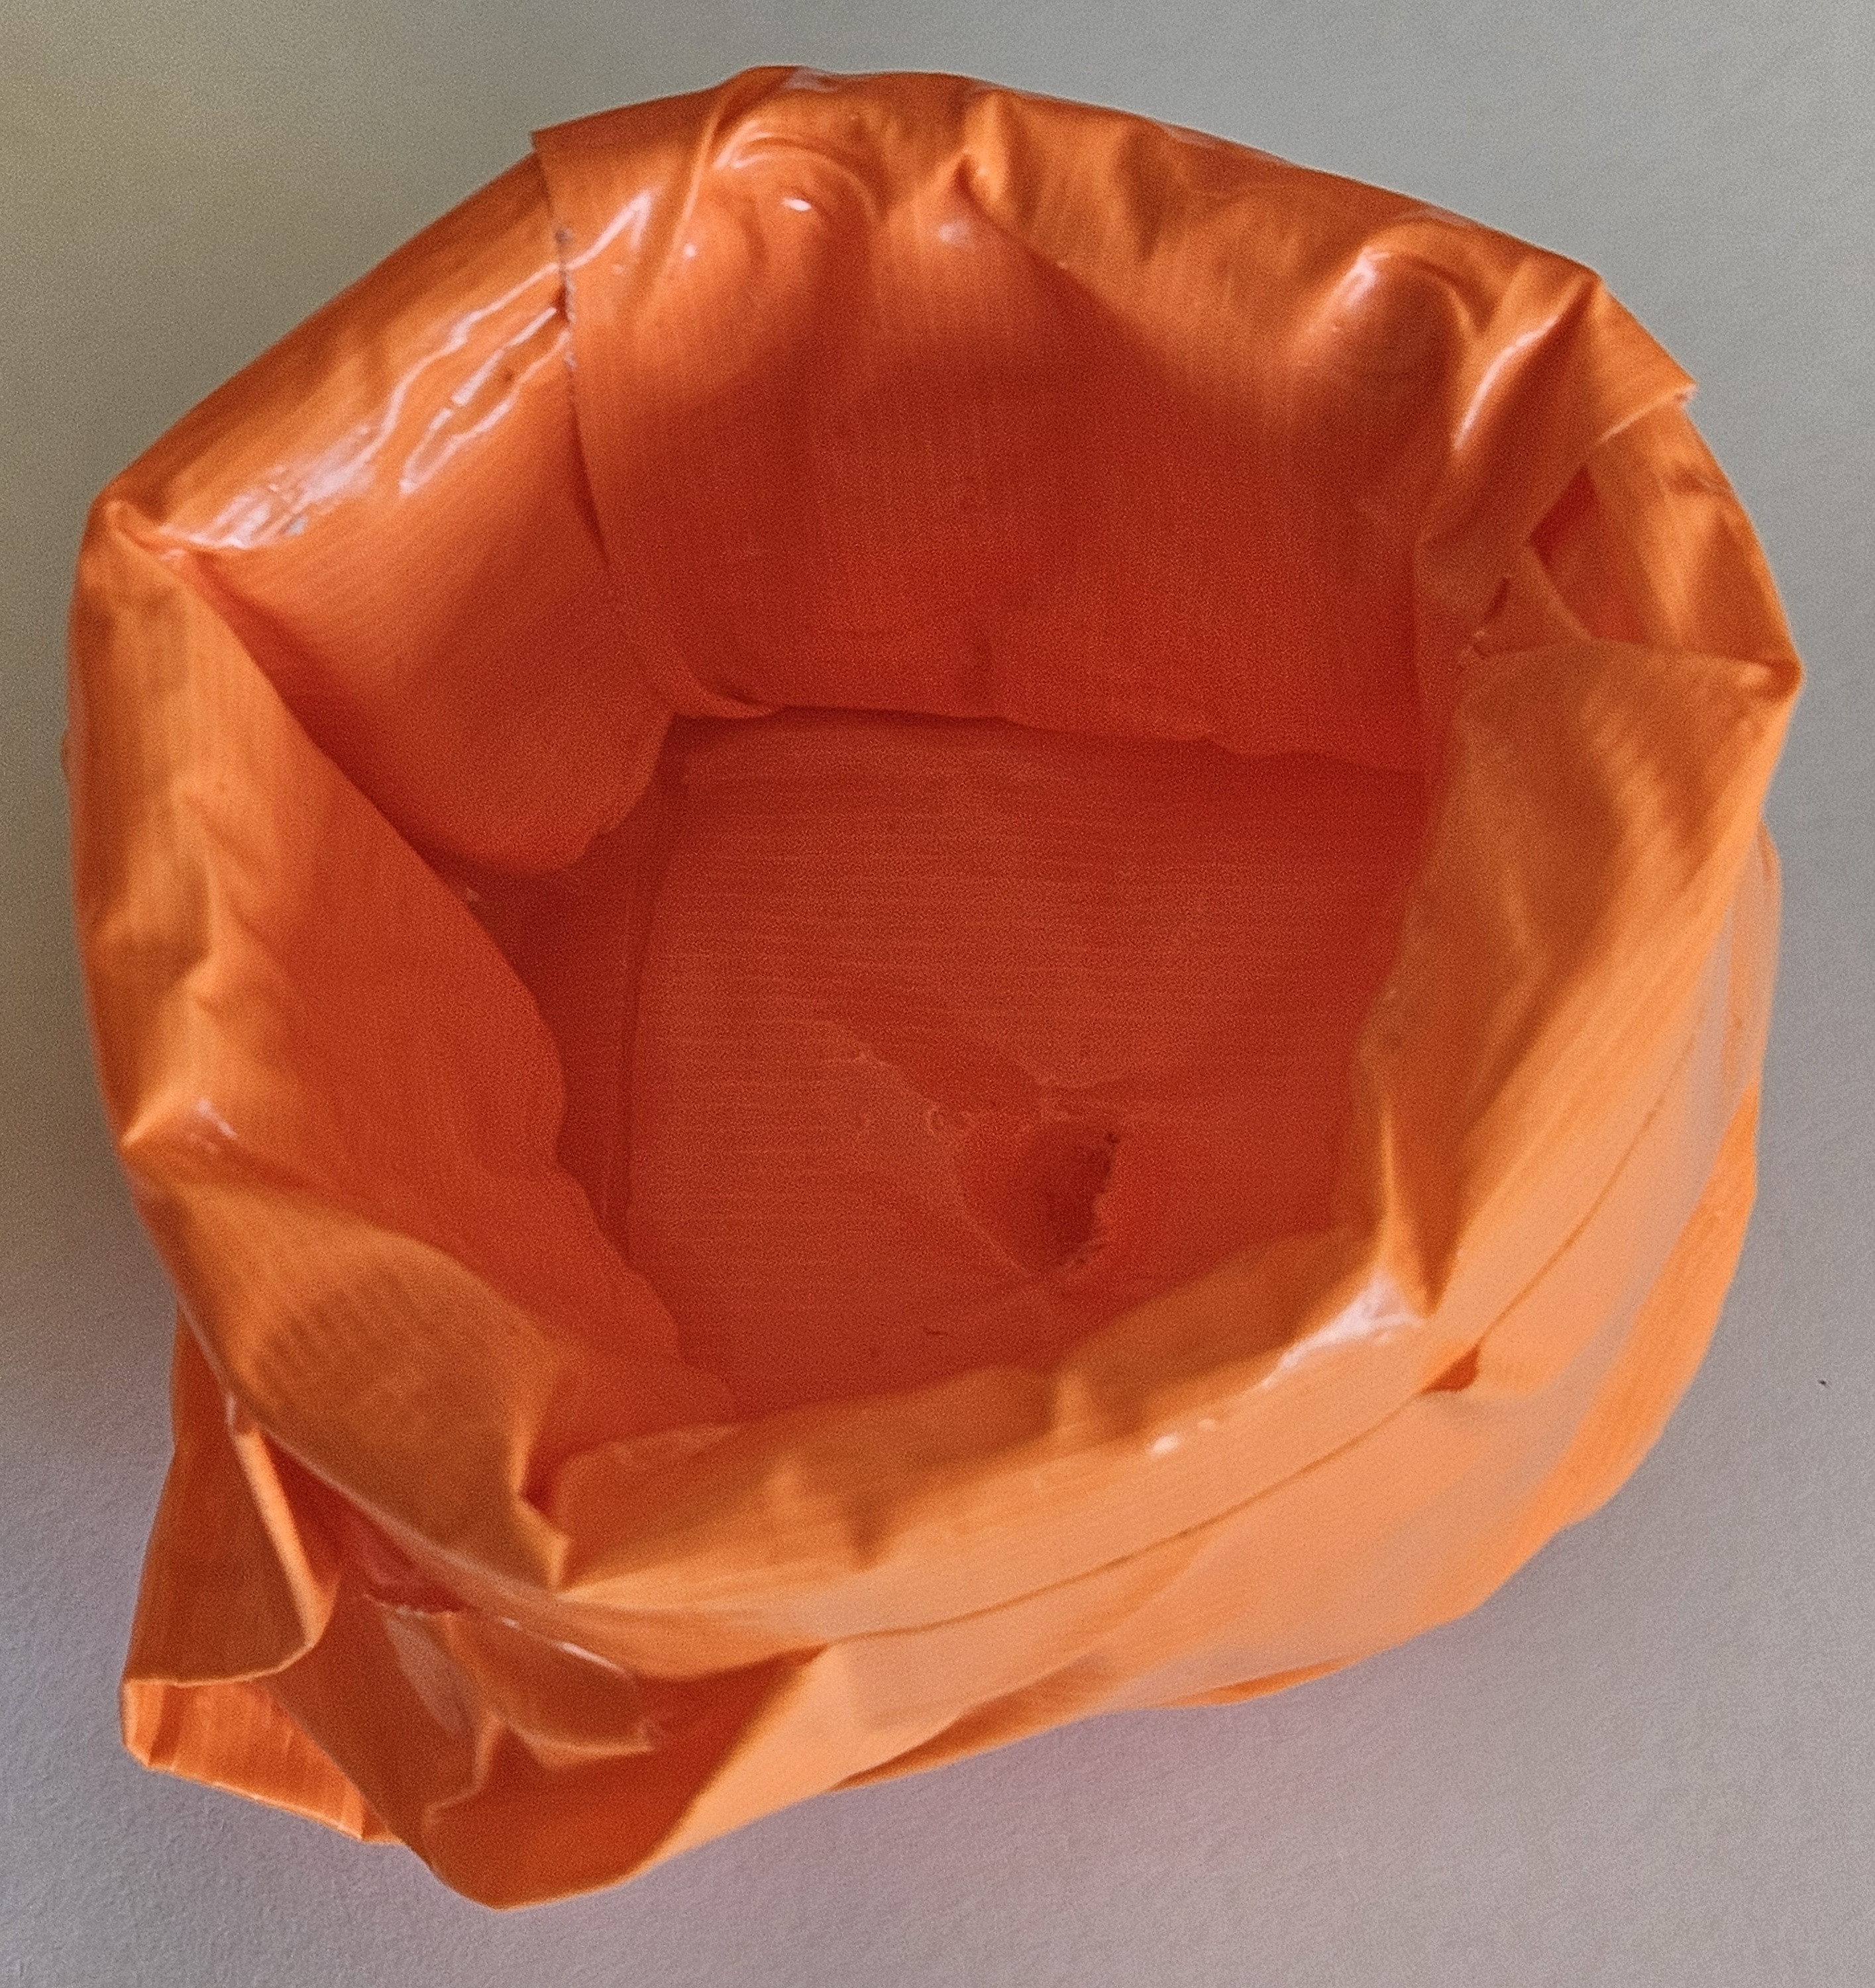
\includegraphics[width=\textwidth]{assets/figures/Interieur_Isolant.jpg}
        \caption{Intérieur de l'isolant thermique}
        \label{fig:Interieur_Isolant}
    \end{minipage}
\end{figure}

\section{Analyse des performances}

Pour évaluer les performances du système de gestion de la température, plusieurs mesures ont été effectuées :  
la température du bain (glacé ou chauffant), la température ambiante, et la température à l’intérieur du module QCM.  
La vitesse de rotation de la pompe a également été enregistrée afin d’étudier son impact sur la température du capteur.

\begin{table}[h!]
\centering
\begin{tabularx}{\textwidth}{|X|X|X|X|X|}
\hline
\textbf{Température du milieu (°C)} & \textbf{Température ambiante (°C)} & \textbf{Température intérieure (°C)} & \textbf{Vitesse (rpm)} & \textbf{$\Delta$ Température (°C)} \\
\hline
75 & 25.4 & 53.3 & 37.6 & 27.9 \\
39 & 26.9 & 28.0 & 2.0 & 1.1  \\
0  & 27.0 & 12.0 & Full & -15.0 \\
\hline
\end{tabularx}
\caption{Mesures de température et de vitesse de pompe}
\end{table}

Le système de gestion de la température est capable de refroidir le capteur jusqu’à 12°C avec de l’eau glacée, et de le chauffer au-delà de 50°C grâce au bain chauffant.  
Il répond donc pleinement aux critères de température requis, soit une plage de 15 à 50°C.